\documentclass[acus]{article}



\usepackage{booktabs} 
\usepackage{longtable}
\usepackage{subfig}
\usepackage{graphicx}

\newcommand{\mfun}[1]{{\bf{#1}}}
\newcommand{\passmethod}[1]{{\texttt{#1}}}
\newcommand{\class}[1]{{\it{#1}}}

\begin{document}

\title{Primer for AT 2.0}
\maketitle
\begin{abstract}
We guide the reader through the basic operations of AT 2.0, starting with lattice creation and manipulation, then
with tracking and optics and beam size computation.
\end{abstract}


\section{Introduction}
AT is a toolbox of functions in Matlab for charged particle beam simulation.  It was created by Andrei Terebilo in the late 1990's.
The original papers \cite{AT1,AT2} still serve as a good introduction to AT.  The AT described in those papers is AT1.3, the latest
version produced by Terebilo.  The next version of AT is considered AT2.0.
Here we provide examples showing some of the changes from AT1.3, but also serving as an introduction for someone just starting
AT.

\subsection{Coordinates}
The 6-d phase space coordinates used in AT are as follows
\begin{equation}
\vec Z = \pmatrix{x\cr \frac{p_x}{P_0} \cr y \cr \frac{p_y}{P_0} \cr \delta \cr c\tau}
\end{equation}
The momenta are defined as
\begin{equation}
p_x = x' P_z  \ \ p_y =  y' P_z
\end{equation}
with $P_z = P_0 (1+\delta)$.  $P_0$ is the reference momentum.  $\tau$ is the time lag relative to
the ideal particle.  In terms of a reference time, it is actually negative: the particles ahead of
the reference particle arrive early.

\section{Creation of Elements and Lattices}
A lattice in AT is a Matlab cell array containing the lattice elements (can be a row or a column).
These elements may be created using element creation functions.  These functions output element structures.  For example, a quadrupole may be created with the function \mfun{atquadrupole}
\begin{verbatim}
>> QF=atquadrupole('QF',0.5,1.2,'QuadMPoleFringePass');
\end{verbatim}
Observing the resulting structure, we see
\begin{verbatim}
QF = 

        FamName: 'QF'
     PassMethod: 'QuadMPoleFringePass'
         Length: 0.5000
          Class: 'Quadrupole'
              K: 1.2000
       PolynomB: [0 1.2000]
       MaxOrder: 1
       PolynomA: [0 0]
    NumIntSteps: 10
\end{verbatim}
We note that the family name of this quadrupole is 'QF' and the pass method is \passmethod{QuadMPoleFringePass}.  The fields following are 
parameters necessary to be able to pass an electron through this quadrupole (i.e., the set of arguments required by the pass
 method).  We now create some other elements needed in a FODO lattice:
 \begin{verbatim}
 >> Dr=atdrift('Dr',0.5);
 >> HalfDr=atdrift('Dr',0.25);
 >> QD = atquadrupole('QD',0.5,-1.2,'QuadMPoleFringePass');
 >> Bend=atsbend('Bend',1,2*pi/40,'PassMethod','BndMPoleSymplectic4Pass');
 \end{verbatim}
In addition to \mfun{atquadrupole} that we already saw, we have created a drift (region with no 
magnetic field), using \mfun{atdrift}.  Besides the family name, the only other needed field is the
length.  Since we split the cell in the center of the drift, we have also created a half drift
element.  The drifts are 0.5 meters long and the half drift is 0.25 meters long.
We have defined a sector dipole, or bend magnet using \mfun{atsbend}.  The family name is 'Bend'.  The
second field is the length of the magnet and we have given it a length of 1 meter.  Next is the bending
angle.  We have defined just an arc of a FODO lattice here, so we don't have to bend by all of $2\pi$
here.  We choose to have 20 total such arcs, for a realistic field strength, and thus we define the
bending angle to be $2*\pi/40$ since there are two bends per cell.  Next, we have defined the pass
method for the bend to be 'BndMPoleSymplectic4Pass'.  This is a 4th order symplectic integrator. 
We outline the integrators in a later section.  

A cell of a FODO lattice may now be constructed as follows
 \begin{verbatim}
 >> FODOcell={HalfDr;Bend;Dr;QF;Dr;Bend;Dr;QD};
 HalfDr];
 \end{verbatim}

As mentioned, this cell is only 1/20 of a FODO lattice. The entire lattice may be created by repeating this cell 20 times as
follows
\begin{verbatim}
>> FODO=repmat(FODOcell,20,1);
\end{verbatim}

Finally, we create a RingParam element and add it to our lattice.  This allows us to give a name to
the lattice and set the ring energy.  This is done as follows:
\begin{verbatim}
>> RP=atringparam('Simple FODO lattice',3e9);
>> FODO=[{RP};FODO];
\end{verbatim}

The energy of a lattice may be retrieved with the function \mfun{atenergy}.  Thus
\begin{verbatim}
>> atenergy(FODO)

ans =

   3.0000e+09
\end{verbatim}
Another way to set the energy of a lattice uses the function \mfun{atsetenergy}.  This puts an 
energy field in all elements and set its to the requested value.  The energy element is required
in the RF cavities and also in the other magnets such as dipoles and quadrupoles in the case that
classical radiation effects are included.

We have now created a valid AT lattice, using drifts, dipoles, 
and quadrupoles.  We will later add some sextupoles to this lattice,
and also an RF cavity, but one could track particles through this lattice, as is.  

For completeness, we list all of the AT element creation functions:
\mfun{ataperture}, \mfun{atbaseelem}, \mfun{atchromMatElem}, \mfun{atcorrector},
\mfun{atdrift}, \mfun{atdampMatElem} (?), \mfun{atdrift}, \mfun{atidtable}, \mfun{atM66}, \mfun{atmarker}, \mfun{atmonitor},
\mfun{atmultipole}, \mfun{atoctupole}, \mfun{atquadrupole}, \mfun{atQuantDiff}, \mfun{atrbend},
\mfun{atrfcavity}, \mfun{atringparam}, \mfun{atsbend}, \mfun{atsextupole}, \mfun{atsolenoid},
\mfun{atthinmultipole}, \mfun{atwiggler}.


\section{Lattice Querying and Manipulation}\label{lattice_query_manip}
There are many parameters in a storage ring lattice.  We need tools to view these parameters and 
to change them.  

We have seen how to concatenate elements to form a lattice.  To extract elements, there are two
approaches, one may use either indices giving the explicit element numbers, or one can use a logical 
mask. Thus, to extract the 4th element of our FODO lattice, (a focusing quadrupole, 'QF'), one may
either write 'FODO{4}'. Likewise, we may also construct a logical mask with
\begin{verbatim}
>> mask=false(1,length(FODOcell));
>> mask(4)=true;
\end{verbatim}
The command 'FODO(mask)' will also give the same 'QF' element.

Next, we describe three important functions for working with AT lattices: \mfun{atgetcells},
\mfun{atgetfieldvalues}, and \mfun{atsetfieldvalues}\footnote{These functions replace the functions
\mfun{findcells}, \mfun{getcellstruct}, and \mfun{setcellstruct} from AT1.3.  These latter functions 
are still supported with backwards compatibility, but are deprecated.}.
\mfun{atgetcells} allows one to find the indices of elements in the lattice searching for 
various criteria.  The second two allow extraction and setting of element parameters.



As a first example of \mfun{atgetcells} let us extract the indices of all of the QF's as follows
\begin{verbatim}
>> QFIndices = atgetcells(FODOcell,'FamName','QF')
\end{verbatim}
which results in
\begin{verbatim}
QFIndices =

     0
     0
     0
     1
     0
     0
     0
     0
     0
\end{verbatim}
where we see the 'QF' at element 4.  To convert this logical mask to an index, use the \mfun{find}
command
\begin{verbatim}
>> find(QFIndices)

ans =

     4
\end{verbatim}

A new feature added to AT 2.0 is element classes.  These are \class{Drift}, \class{Bend}, \class{Quadrupole}, \class{Sextupole}, \class{Octupole}, \class{Multipole}, \class{ThinMultipole}, 
\class{Wiggler}, \class{KickMap}, \class{RFCavity}, \class{QuantDiff}, \class{Monitor}, \class{Corrector}, \class{Solenoid}, 
\class{Matrix66}, \class{RingParam}.
This allows us to get the indices for all of the quadrupoles with the command
 \begin{verbatim}
>> QuadIndices = atgetcells(FODO,'Class','Quadrupole')
\end{verbatim}
with the result
\begin{verbatim}
>> find(QuadIndices)

ans =

     5
     9
    14
    18
    23
    27
    32
    36
    41
    45
    50
		...
\end{verbatim}
showing the indices of both 'QF' and 'QD' in the FODO cell.  

The reader can look further into the help for \mfun{atgetcells} by typing
\begin{verbatim}
>> help atgetcells
\end{verbatim}
to see other ways this function can be used, including the use of matching 
regular expressions.

The \mfun{atgetfieldvalues} command may be used to extract the fields with the elements.  For example the quadrupole strengths may be 
retrieved using the command
 \begin{verbatim}
>> Kvals=atgetfieldvalues(FODO,QuadIndices,'PolynomB',{1,2});
\end{verbatim}
The \mfun{setcellstruct} command may be used to set the values of parameters.  As a simple example, we may add some
random errors to all the quadrupoles strengths:
 \begin{verbatim}
>> Kvalserr=Kvals+0.2*(rand(length(Kvals),1)-0.5);
>> FODOerr=atsetfieldvalues(FODO,QuadIndices,'PolynomB',{1,2},Kvalserr);
\end{verbatim}
Note that the output of \mfun{setcellstruct} is another lattice structure, which here we call 'FODOerr' which has the
quadrupole strengths 'Kvalserr'.  Now we have both 'FODO' and 'FODOerr' in the Matlab workspace and we can examine
them or do calculations for comparison.

Suppose we would like to plot the quadrupole strengths along the lattice.  We first need to find the
longitudinal, $s$
position of each quadrupole.  This may be done with the function \mfun{findspos}:
\begin{verbatim}
>> quadspos = findspos(FODO,QuadIndices);
\end{verbatim}
The quadrupole strengths of 'FODO' and 'FODOerr' may now be plotted with
\begin{verbatim}
>> plot(quadspos,Kvals,'*r',quadspos,Kvalsb,'*b');
\end{verbatim}
The plot is shown in Figure \ref{quadplot}.
\begin{figure}[htb]
\centering
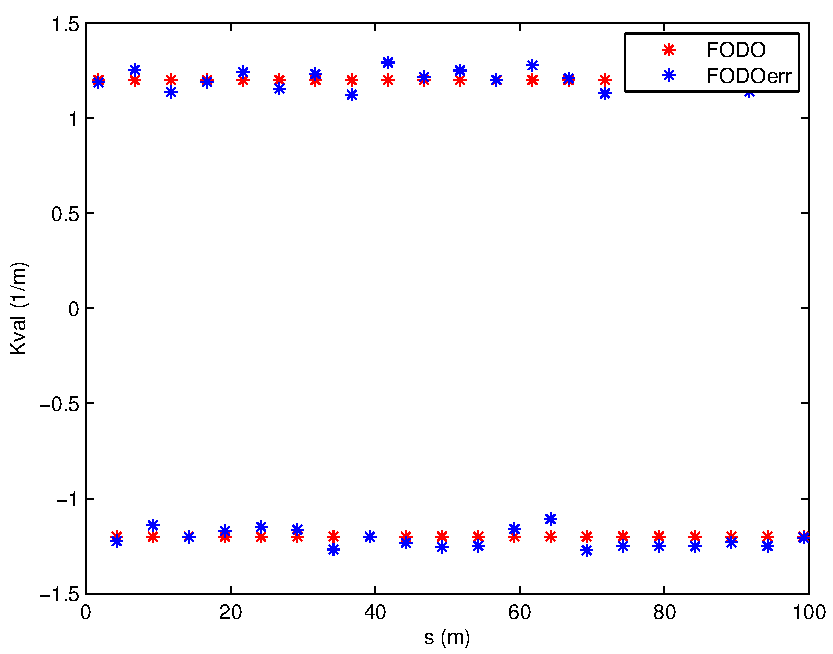
\includegraphics[scale=0.5]{quadplot.pdf}
\caption{Plot of quadrupole strengths for FODO lattice with and without errors.}
\label{quadplot}
\end{figure}

\section{Tracking}
Once a lattice is defined, electrons may be tracked through it.  \mfun{ringpass} is the
function that does the tracking.  An example of its use is as follows:
\begin{verbatim}
>> nturns=200;
>> Z01=[.001;0;0;0;0;0];
>> Z02=[.002;0;0;0;0;0];
>> Z03=[.003;0;0;0;0;0];
>> Z1=ringpass(FODO,Z01,nturns);
>> Z2=ringpass(FODO,Z02,nturns);
>> Z3=ringpass(FODO,Z03,nturns);
>> plot([Z1(1,:); Z2(1,:); Z3(1,:)]',[Z1(2,:); Z2(2,:); Z3(2,:)]','.')
\end{verbatim}
The plot is shown in Figure \ref{trackPlot}.
\begin{figure}[htb]
\centering
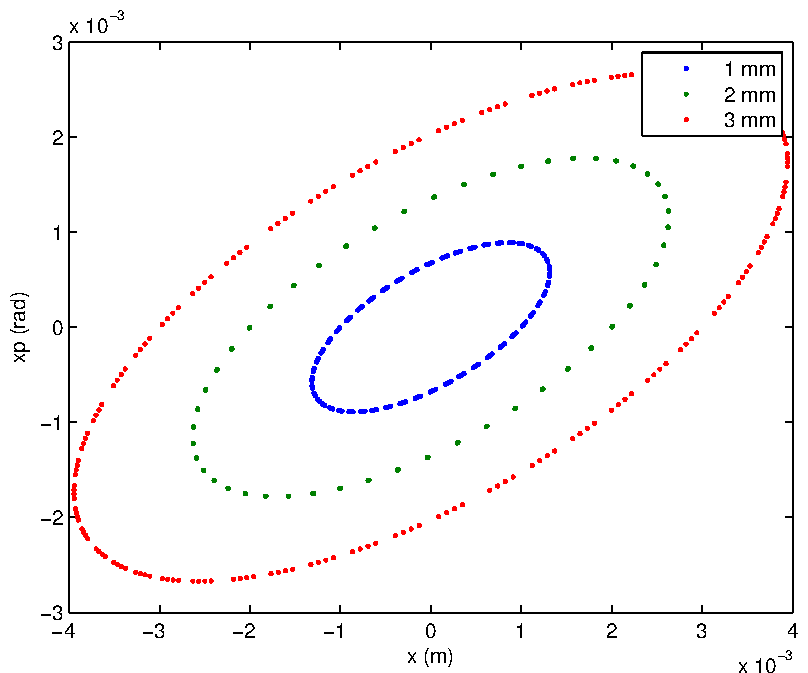
\includegraphics[scale=0.5]{trackPlot.pdf}
\caption{Tracking results in FODO lattice.}
\label{trackPlot}
\end{figure}
In this example, we started with one initial condition, and all subsequent 
turns
are returned by ringpass.  We may also start with multiple initial conditions:
\begin{verbatim}
>> Z0=[.001;0;0;0;0;0]*(1:3);
>> Z200=ringpass(FODO,Z0,nturns);
\end{verbatim}
Examining the variable Z200, we find
\begin{verbatim}
>> whos Z200
  Name      Size             Bytes  Class     Attributes

  Z200      6x600            28800  double
\end{verbatim}
The structure of this matrix is that the first three columns are the results of tracking
for one turn the three initial conditions.  The following columns are likewise grouped in
threes with the subsequent results of tracking further turns.  We may retrieve the same results
as we had previously by extracting every third column vector as follows:
\begin{verbatim}
>> ZZ1=Z200(:,1:3:3*nturns);
>> ZZ2=Z200(:,2:3:3*nturns);
>> ZZ3=Z200(:,3:3:3*nturns);
\end{verbatim}
Now the same plot as in Figure \ref{trackPlot} results from the plot command
\begin{verbatim}
>> plot(ZZ1(1,:),ZZ1(2,:),'.r',ZZ2(1,:),ZZ2(2,:),'.b',ZZ3(1,:),ZZ3(2,:),'.k')
\end{verbatim}
Another way to process the output of ringpass with multiple initial particles uses
the \mfun{reshape} command
\begin{verbatim}
>> ZZ200=reshape(Z200,6,3,nturns);
>> ZZZ1=ZZ200(:,1,:);
>> ZZZ2=ZZ200(:,2,:);
>> ZZZ3=ZZ200(:,3,:);
\end{verbatim}
This can be a convenient approach to process the results when many initial 
conditions are tracked.

\section{Computation of beam parameters}
Now that particles can be tracked through the lattice, we can use the
tracking to understand different properties of the lattice.  First, we
would like to understand the linear properties such as Twiss
paramers, tunes, chromaticities, etc.
These can all be calculated with the function atlinopt.
\begin{verbatim}
>> [param,t,c]=atlinopt(FODO,0,1);
\end{verbatim}
Note first the three inputs.  The first is the FODO lattice we 
have created.  The second argument of 0 says we want to compute
the linear optics on energy with $\delta=0$.  The third argument
is a list of indices for where we want to compute the different 
linear optics parameters.  The 1 says that we will just compute it
at the beginning of the lattice.  

Next, there are three outputs, the first is the optics parameters,
evaluated at the positions requested.  The t gives the horizontal and
vertical tunes and the c gives the chromaticity.  Examining first the
tunes and chromaticities, we find
\begin{verbatim}
>> t,c

t =

    0.2867    0.6990


c =

   -1.8248   -1.7404
\end{verbatim}
which tells us the tunes are $\nu_x = 0.2867$ and $\nu_y = 0.6990$ and the 
chromaticities are $\xi_x = -1.8248$, $\xi_y = -1.7404$.

How did AT calculate these quantities?  Without digging into the
details of atlinopt, you could still figure it out, just based on
the ability to track with the ringpass function.  In fact, AT computes
the one turn transfer matrix by tracking several initial conditions and
interpolating.  The one turn transfer matrix (here we focus on 4x4) is 
computed with the function findm44 contained within atlinopt.  
Calling this on the FODO lattice, we find
\begin{verbatim}
>> findm44(FODO,0)

ans =

    0.3140    1.1838         0         0
   -0.4988    1.3040         0         0
         0         0   -2.2637   -6.2810
         0         0    0.7523    1.6457
\end{verbatim}
The 0 as the second argument tells us to compute with $\delta=0$.
We note that the ring is uncoupled, and computing the eigenvalues of
submatrices, we derive the tunes reported in atlinopt above.

Computing the tunes with varying initial $\delta$ allows the 
computation of the chromaticity.  

Now, suppose we would like to change the tunes in our FODO lattice.  
We know that we should change the quadrupole strengths, but we may
not know exactly what values to use.

Here we reach the question of tuning.  How do we set the parameters for
these quadrupoles in order to correct the tunes?
In principle we have the tools that we need.  We can set the values
of the quadrupoles using the function \mfun{setcellstruct} and then
recompute the chromaticity with \mfun{atlinopt}.  But we still don't know what 
values to actually give the quadrupoles.  One could compute the
value, or instead use an optimization routine to vary the values
until the correct output tunes are achieved.  This is the
approach followed with the function \mfun{atfittune}.  

This allows you to vary quadrupole strengths until the desired tune
values are reached.  It is used as follows 
\begin{verbatim}
>> FODO2=atfittune(FODO,[0.15,0.75],'QF','QD');
\end{verbatim}
which would set the tunes to $\nu_x = 0.15$ and $\nu_y = 0.75$ using
the quadrupoles QF and QD. When we actually try this, and compute the
linear optics, we find the result
\begin{verbatim}
>> [param2,t2,c2]=atlinopt(FODO2,0,1); t2
>> t2 =

    0.1472    0.7503
\end{verbatim}
We see that the requested values have almost been reached, but not exactly.
A second call to \mfun{atfittune} gives
\begin{verbatim}
>> FODO2=atfittune(FODO2,[0.15,0.75],'QF','QD');
>> [param2,t2,c2]=atlinopt(FODO2,0,1); t2
>> t2 =

    0.1500    0.7500
\end{verbatim}
Giving satisfactory results for the tunes.

Now, in case you have some experience with storage ring dynamics,
you will know that these negative chromaticity values will lead
to instability and thus our FODO lattice, as is, is not acceptable.
To fix this problem, we add sextupoles to our lattice.
We define a focusing and defocussing sextupoles (0.1 meter long)
as follows:
\begin{verbatim}
SF=atsextupole('SF',0.1,1);
SD=atsextupole('SD',0.1,-1);
\end{verbatim}
Now we want to add these to the lattice at locations where they will
be effective.  We will put them in the middle of the 0.5 meter drift
sections: SF before the QF and SD before the QD.  Thus, we need a 
new drift of 0.2 meters long:
\begin{verbatim}
p2Dr=atdrift('Dr',0.2);
\end{verbatim}
And now we can define our lattice cell with sextupoles as follows
\begin{verbatim}
FODOcellSext=[{HalfDr};{Bend};{p2Dr};{SF};{p2Dr};...
{QF};{Dr};{Bend};{p2Dr};{SD};{p2Dr};{QD};{HalfDr}];
FODOSext=repmat(cell,20,1);
\end{verbatim}

Now that we have added the sextupoles, we need to know how to set them.
Back to the chromaticity, we now fix the chromaticities, using the function
\mfun{atfitchrom}.  This function works analogously to \mfun{atfittune} except
the sextupoles are varied instead of the quadrupoles to fit the chromaticity.
Applying this function (twice to get a more precise result):
\begin{verbatim}
FODOSext=atfitchrom(FODOSext,[0.5 0.5],'SF','SD');
FODOSext=atfitchrom(FODOSext,[0.5 0.5],'SF','SD');
\end{verbatim}

After changing the tunes and fixing the chromaticities, we find
\begin{verbatim}
>> [paramS,tS,cS]=atlinopt(FODOSext,0,1);tS,cS
tS =

    0.1500    0.7500


cS =

    0.4996    0.4993
\end{verbatim}

You may have noticed that we bypassed the initial output of \mfun{atlinopt},
the parameters.  This contains linear optics parameters that vary around the ring.
These are the Twiss parameters, dispersions, phase advance, and coupling parameters.
To compute these around the ring, we need to give the indices for the reference points.
To compute them at all lattice elements, we call
\begin{verbatim}
>> [paramAll,t2,c2]=atlinopt(FODOSext,0,1:length(FODOSext)+1);
\end{verbatim}
Examining 'paramAll', we find
\begin{verbatim}
>> paramAll
paramAll = 

1x261 struct array with fields:

    ElemIndex
    SPos
    ClosedOrbit
    Dispersion
    M44
    gamma
    C
    A
    B
    beta
    alpha
    mu
\end{verbatim}
'ElemIndex' is the set of indices where the optics parameters are defined.  'SPos'
is the set of $s$ positions.  'ClosedOrbit' is the $x,x',y,y'$ of the closed orbit
at each element location.  'Dispersion' gives the horizontal and vertical dispersion
and dispersion derivative.  'M44' is the local $4\times 4$ transfer matrix.  'gamma',
'C','A', and 'B' are coupling parameters\cite{SaganRubinCoupling}. 'beta' gives the horizontal and vertical beta
functions. 'alpha' gives the Twiss parameters $\alpha_{x,y}$ and 'mu' gives the phase
advances (times $2\pi$).

Let us use these results to plot the beta functions around the ring.
\begin{verbatim}
>> beta=cat(1,paramAll.beta);
>> betax=beta(:,1);
>> betay=beta(:,2);
>> spos=cat(1,paramAll.SPos);
>> figure
>> plot(spos,betax,'-r',spos,betay,'-b');
>> xlabel('s (m)');
>> ylabel('beta (m)');
>> legend('betax','betay');
\end{verbatim}
The result is shown in Figure \ref{FODOBetaPlot}.
\begin{figure}[htb]
\centering
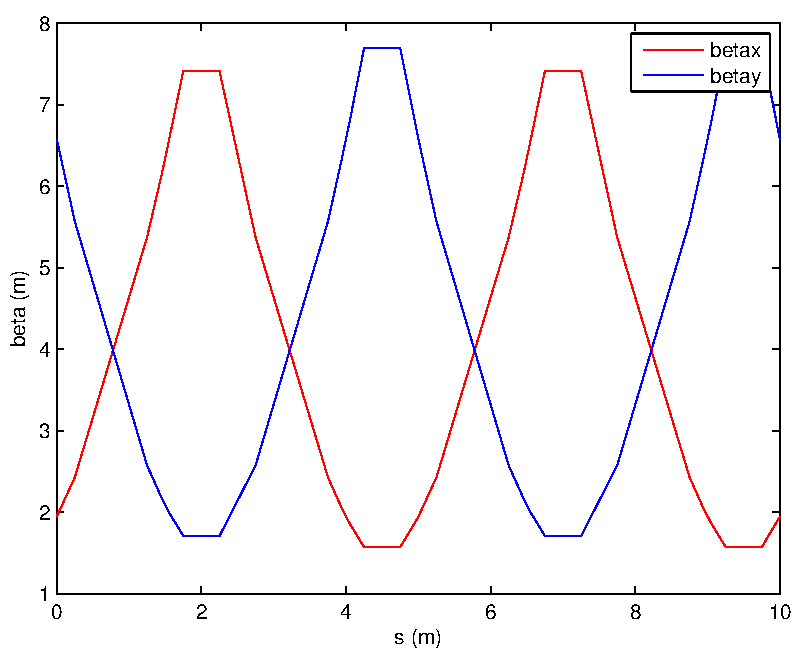
\includegraphics[scale=0.5]{FODOBetaplot.pdf}
\caption{Plot of FODO lattice beta functions.}
\label{FODOBetaPlot}
\end{figure}


We may also plot the lattice parameters using a dedicated function called \mfun{atplot}
with the command
\begin{verbatim}
atplot([FODOcellSext;FODOcellSext]);
\end{verbatim}
The result is shown in Figure \ref{FODOATPlot}. Note that the magnets are displayed below
the function, giving a convenient visualization.  Also note that the lattice functions are smoother
than those we see in Figure \ref{FODOBetaPlot}.
They have been computed at more positions, but slicing the magnets in the atplot function.

\begin{figure}[htb]
\centering
\includegraphics[scale=0.5]{FODOATPlot.pdf}
\caption{Plot result of \mfun{atplot} on the FODO lattice showing beta functions and dispersion,
smoothed via element slicing and also including magnet represenation.}
\label{FODOATPlot}
\end{figure}

\subsection{Beam sizes}
The parameters computed thus far use only the tracking through the lattice, with no radiation
effects.  In reality, for electrons, we know that there are radiation effects which cause
a damping and diffusion and determine equilibrium emittances and beam sizes.
This is computed in AT using the Ohmi envelope formalism.  A simple interface to this code
is provided via the function \mfun{atx} which gives the linear optics parameters we have
just computed, and also the beam sizes.

In order to use \mfun{atx}, we first need to make sure the beam is stable longitudinally as 
well, requiring us to add an RF cavity to our FODO lattice.  This is done with the command
\begin{verbatim}
>> RFC=atrfcavity('RFCav');
\end{verbatim}
and the cavity is added to the lattice
\begin{verbatim}
FODOSextRF=[{RFC};FODOSext];
\end{verbatim}
Now, we need to set the values of the RF cavity.  This can be done with the 
function \mfun{atsetcavity} as follows
\begin{verbatim}
FODOSextRF=atsetcavity(FODOSextRF,5e5,0,100);
\end{verbatim}
which says that the RF cavity has a voltage of 5MV and harmonic number of 100.

We may now call the function \mfun{atx} as follows
\begin{verbatim}
>> [BEAMDATA,PARAMS]=atx(FODOSextRF);
\end{verbatim}
with the results
\begin{verbatim}
             ll: 100.0000
           alpha: 0.0419
       fractunes: [0.2199 0.9178]
       fulltunes: [5.2199 4.9178]
             nuh: 5.2199
             nuv: 4.9178
    chromaticity: [0.5000 0.5083]
     dampingtime: [0.0536 0.0478 0.0228]
         espread: 3.3112e-04
         blength: 0.0121
    modemittance: [3.3655e-08 7.3019e-37 3.9995e-06]
          energy: 1.0000e+09
              fs: 5.4812e+04
           eloss: 1.3901e+04
    synchrophase: 0.0278
      momcompact: 0.0419
\end{verbatim}
We see that our FODO lattice has an emittance of 33.66 nm, an energy spread of $3.3\times 10^{-4}$
and a bunch length of 12.1 mm.


\begin{thebibliography}{4}

\bibitem{AT1}
A. Terebilo \emph{Accelerator Toolbox for Matlab}, SLAC-PUB 8732 (May 2001)
\bibitem{AT2}
A. Terebilo, \emph{Accelerator Modeling with Matlab Accelerator Toolbox}, PAC 2001 Proceedings
\bibitem{ATIpac}
B. Nash et. al. \emph{New Functionality for Beam Dynamics in Accelerator Toolbox}, IPAC 2015
\bibitem{SaganRubinCoupling} 
D. Sagan, D. Rubin, \emph{Linear Analysis of Coupled Lattices}, Phys. Rev. Special Topics - Accelerators and Beams, Vol 2,(1999)

\end{thebibliography}

\end{document}

